\documentclass{article}
\usepackage[utf8]{inputenc}

\newcommand\ddfrac[2]{{\displaystyle\frac{\displaystyle #1}{\displaystyle #2}}}

\title{COP290-A1}
\author{Sayam Sethi 2019CS10399 \\ Mallika Prabhakar 2019CS50440 }
\date{March 2021}

\usepackage{natbib}
\usepackage{graphicx}

\begin{document}

\maketitle

\section{Metrics}
%define your utility and runtime metrics here
For any software, we need to consider a lot of aspects like accuracy, hardware resources, privacy, latency, etc. Improving one aspect might hamper the second aspect hence there is a trade-off. To analyse this trade-off, we have to use certain metrics to compare different approaches and optimisations. The utility function and runtime metric used for this assignment are described as follows-

\subsection{Penalty Function}
A penalty function is considered which takes into account both deviation in error and execution time into account.

\textbf{Specifications:} The penalty function was made keeping in account that higher reduction in runtime leads to a larger error and hence, if the runtime reduction is more, the contribution of the error to the function should be reduced. The final function considered was:
\begin{center}
    $\ddfrac{1 + \mathit{mean}(\mathit{square}(10000\cdot\mathit{diff}(\mathit{queueDensityBaseline}, \mathit{queueDensityCurr})))}{1 + \frac{\mathit{baseRuntime} - \mathit{currentRuntime}}{\mathit{baseRuntime}}}$
\end{center}
Initially many variations were explored in which the numerator and denominator were raised to different powers, however, they led to highly similar graphs and not much difference was observed in the relative trends. Hence, the simple ratio was finally considered.

\subsection{Runtime Metric}
% @TODO :sadface
\textbf{Specifications:}


\section{Methods}
Following methods are the ones which we implemented and considered with respect to the sub-task 2 implementation:

\subsection{Sub-sampling frames}
Main idea behind sub-sampling is to process every $x\textsuperscript{th}$ frame i.e. if the last frame was $N$, the next frame to be processed will be the one at position $N+x$. In our implementation, we skip the processing of next $x-1$ frames by using a for loop to go through the frames in the designated video.

\subsection{Resolution reduction}
Resolution reduction is performed to decrease the processing time of various functions called on the frame matrix by reducing it size while trying to keep the error minimum. In our implementation, we reduce the resolution of each dimension of the video by a factor of $x$ and process it.

\subsection{Spatial threading}
Splitting work spatially by allotting different sections of every frame matrix to different threads is a lucrative method to spread the processing load. The reference frame is read and broken into $x$ segments which is stored in a struct. During the processing of each frame, the frame is directly passed to the thread functions, where based on the $thread\_id$, the corresponding segment is obtained and sum of the ``white pixels" obtained. In the same loop, the threads are joined and the values obtained are added and the result reported for that thread.

\subsection{Temporal threading}
This method involves reading multiple frames one after the other and then processing all of them at the same time. In a single iteration of the loop, $x$ frames are read and corresponding threads created and the frame passed to it. 

\section{Trade-off analysis}
While building a software, our purpose is to not only maximise the accuracy but also the other user and hardware specific features like latency in computation, temperature of the CPU unit and other hardware, security and privacy of data, etc. For this assignment, we have mainly considered the computation speed and accuracy for trade-off analysis.

\subsection{Sub-sampling frames}
Intuitively, the execution time is expected to decrease with a larger sub-sampling parameter. Indeed, this is what actually happens:
\begin{center}
    \makebox[\textwidth]{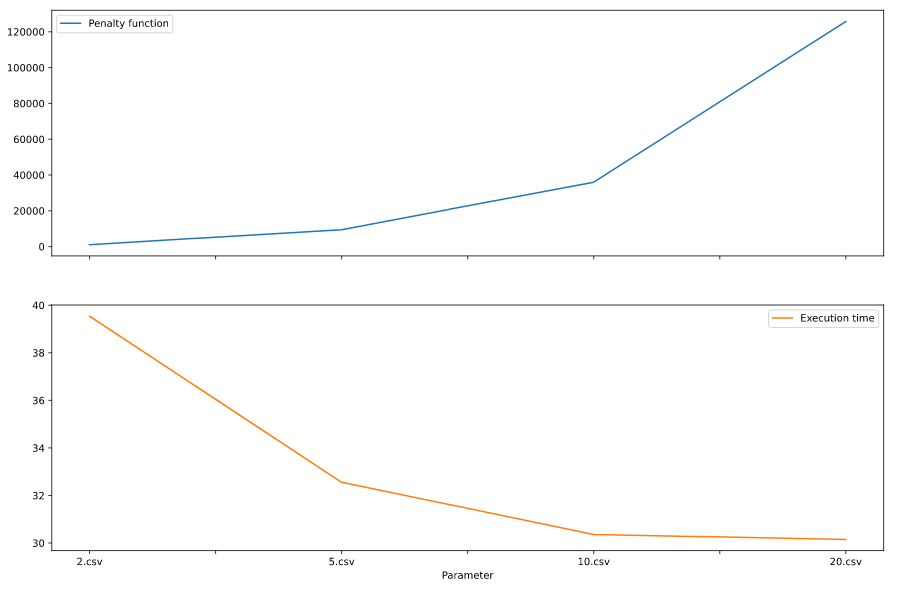
\includegraphics[width=1.25\textwidth]{Graphs/subsampling.png}}
    Sub-sampling graphs
\end{center}
From the graph, we observe that the execution time decreases by a large extent initially and then saturates at about $30s$. The penalty function also, as expected, increases with a larger sub-sampling factor. If one permits slight tolerance, then sub-sampling factor of $5$ is the most optimal, since there is a huge reduction in execution time, but a very small value of penalty function.

\subsection{Resolution reduction}
In this case again, we expect the execution time to reduce with the increase in the resolution parameter. The graph conveys the same results:
\begin{center}
    \makebox[\textwidth]{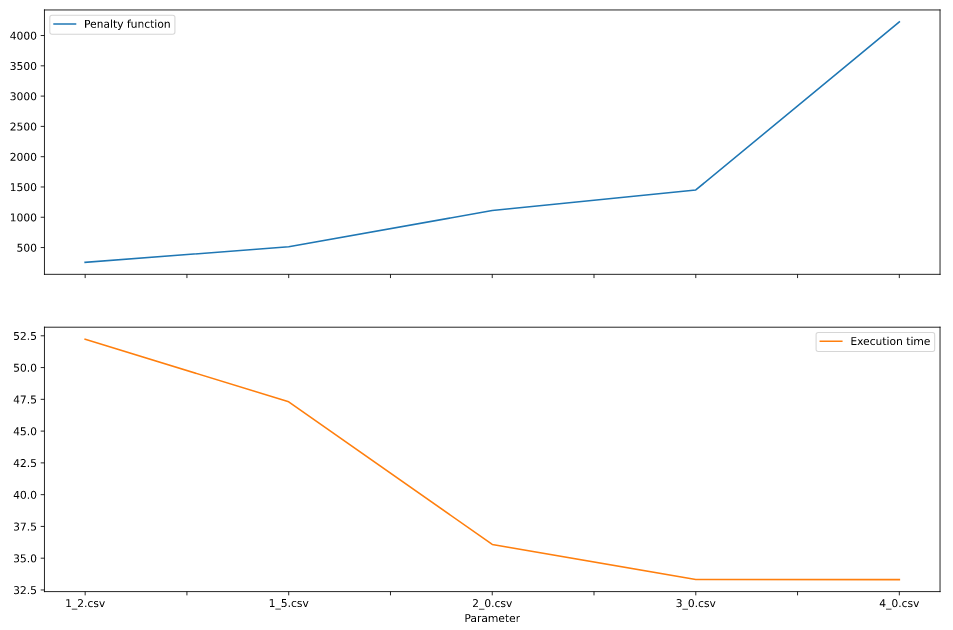
\includegraphics[width=1.25\textwidth]{Graphs/resolution.png}}
    Resolution graphs
\end{center}
Initially, there is a slight increase since resizing is not a constant time operation. Also, the reduction in the execution time is relatively lesser for smaller scaling factor and decreases suddenly. The execution time saturates in this too, at about $32s$. The penalty function increases considerably with higher scaling factor and shoots up beyond a factor of $3$. Thus, to get optimal results with a small tolerance, scaling factor under $1.5$ should be preferred, and to get considerable reduction in execution time but a relatively higher tolerance is acceptable, then a scaling factor between $1.5$ and $2$ is desirable.

\subsection{Spatial threading}
In this method, it is not easy to guess if execution time will improve with more threads or not since splitting each frame into segments has a large contribution to the execution time too. On running the code and plotting the graphs, we get:
\begin{center}
    \makebox[\textwidth]{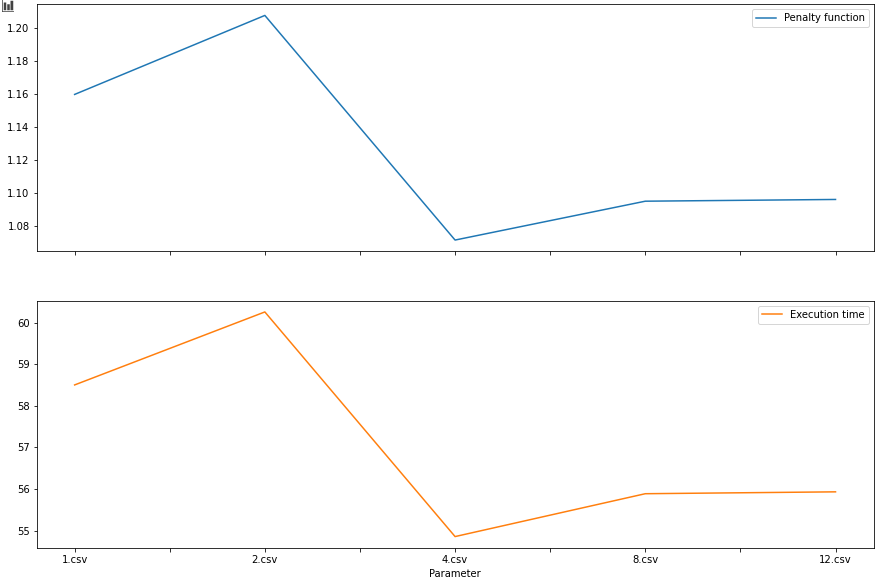
\includegraphics[width=1.25\textwidth]{Graphs/spatialThreading.png}}
    Spatial threading graphs
\end{center}
Large variation is observed in the execution time with different number of threads. The execution time initially increases since creating more matrices takes more time than what is saved because of dividing the work into threads. On increasing the threads further, the execution time decreases since the time saved due to parallel processing is more than the time increase due to forming segments. The time taken increases slightly on increasing the number of threads since creating and joining larger number of threads is time consuming.\par
The penalty function is dependent only on the execution time since the error encountered is zero (and hence the numerator equals $1$). Thus, the most optimal number of threads in spatial threading is $4$, which gives the least execution time. However, it is to be noted that this is still more than the execution time that is obtained without using any threads.

\subsection{Temporal threading}
In this method, multiple frames are processed at once, hence, the execution time is expected to decrease with larger number of threads. This is what the graph shows:
\begin{center}
    \makebox[\textwidth]{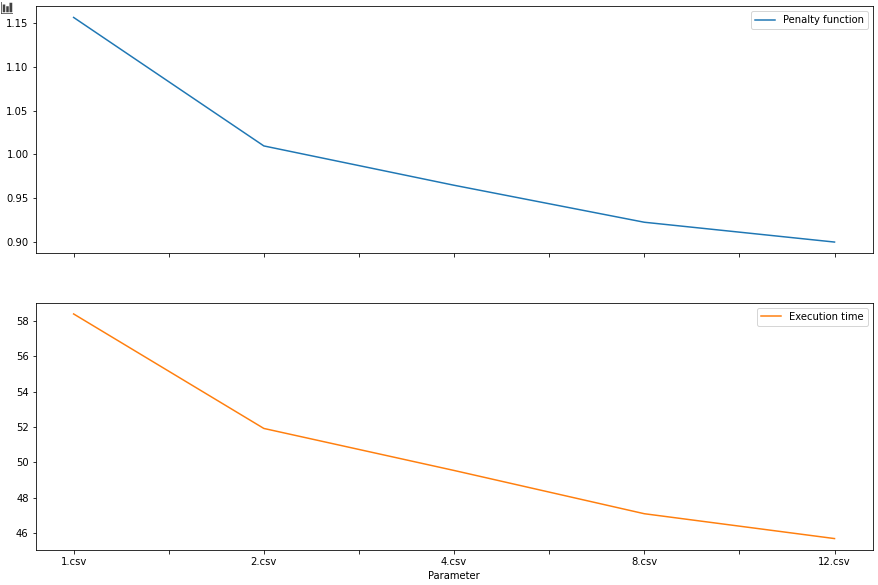
\includegraphics[width=1.25\textwidth]{Graphs/temporalThreading.png}}
    Temporal threading graphs
\end{center}
Initially the execution time is larger compared to the baseline code since creating threads takes time. Also, the reduction in the execution time is clearly visible with a decrease in the number of threads. Additionally, the reduction in execution time gradually becomes lesser. Similar to spatial threading, the penalty function is dependent only on the runtime since the error is zero and hence the numerator equal to $1$. The most optimal parameter would be to use as many threads as possible that can be simultaneously processed by the computer ($12$ in the case of the device used to perform testing on).

\subsection{Note on CPU Usage}
The execution of only the main function is not directly a single thread operation and the processor uses multiple threads even for a single thread code:
\begin{center}
    \makebox[\textwidth]{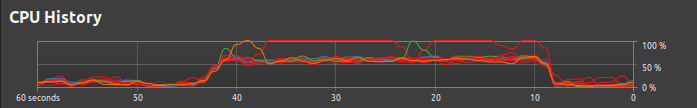
\includegraphics[width=1.25\textwidth]{Graphs/nonThreadedCPU.png}}
    CPU usage on running a single thread code
\end{center}
In the previous image, the average CPU usage increased to over $60\%$ across all threads even though it was a single thread operation. Also, it can be noticed that at any point of time, there is one core which has close to $100\%$ usage and that thread keeps on changing.\par
For a multi-threaded code, the CPU usage looks as follows:
\begin{center}
    \makebox[\textwidth]{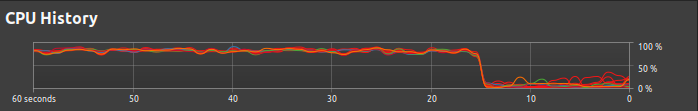
\includegraphics[width=1.25\textwidth]{Graphs/threadedCPU.png}}
    CPU usage on running a multi-thread code ($4$ threads)
\end{center}
Here, all the $12$ cores have a really high average CPU usage, over $80\%$, even though only $4+1$ (additional threads + main thread) threads were used. This can be possibly explained using the fact that the exact same set of cores is not used to create the threads, since breaking and joining of the threads happens multiple times throughout the code.

% wow
\end{document}
%nice yay